% !TEX program = xelatex
% !TEX encoding = UTF-8 Unicode
% !TEX spellcheck = de_DE

% --------------------------------------------------------------------------- %
% Poster template for Institute of Telematics.      						  %
% --------------------------------------------------------------------------- %
% Created with Brian Amberg's LaTeX Poster Template. Please refer for the     %
% attached README.md file for the details how to compile.				      %
% --------------------------------------------------------------------------- %
% $LastChangedDate:: 2017-08-03 18:00:00 +0200 (V, 12 szept. 2017)          $ %
% $LastChangedRevision:: 129                                                $ %
% $LastChangedBy:: allner                                                   $ %
% $Id:: poster.tex 128 2011-09-11 08:57:12Z rlegendi                        $ %
% --------------------------------------------------------------------------- %


\documentclass[a0paper,portrait]{baposter}

\usepackage[utf8]{inputenc}
\usepackage{relsize}		% For \smaller
\usepackage{url}			% For \url
\usepackage{epstopdf}	% Included EPS files automatically converted to PDF to include with pdflatex
\usepackage{verbatimbox}
\usepackage{enumitem}
\usepackage{wrapfig}

\usepackage{setspace}
\usepackage{uzlcolor}
\usepackage[ngerman]{babel}
\usepackage{blindtext}

\usepackage[style=ieee,doi=false,maxbibnames=3]{biblatex}
\addbibresource{references.bib}

%%% Myriad Pro Font - %%%%%%%%%%%%%%%%%%%%%%%%%%%%%%%%%%%%%%%%%%%%%%%%%%%%%%%%%
\usepackage{fontspec}
\defaultfontfeatures{Mapping=tex-text,Scale=MatchLowercase}
\setmonofont{Myriad Pro}
\setmainfont[
BoldFont={Myriad Pro}, 
ItalicFont={Myriad Pro},
BoldItalicFont={Myriad Pro}
]{Myriad Pro}
\setsansfont{Myriad Pro}



%%% Global Settings %%%%%%%%%%%%%%%%%%%%%%%%%%%%%%%%%%%%%%%%%%%%%%%%%%%%%%%%%%%
\graphicspath{{pix/}}	% Root directory of the pictures 
\tracingstats=2			% Enabled LaTeX logging with conditionals

\newcommand{\localtextbulletone}{\textcolor{uzl_orange_2}{\raisebox{0.2ex}{\rule{1.2ex}{1.2ex}}}}
\renewcommand{\labelitemi}{\localtextbulletone}

%%%%%%%%%%%%%%%%%%%%%%%%%%%%%%%%%%%%%%%%%%%%%%%%%%%%%%%%%%%%%%%%%%%%%%%%%%%%%%%%
%%% Utility functions %%%%%%%%%%%%%%%%%%%%%%%%%%%%%%%%%%%%%%%%%%%%%%%%%%%%%%%%%%

%%% Save space in lists. Use this after the opening of the list %%%%%%%%%%%%%%%%
\newcommand{\compresslist}{
	\setlength{\itemsep}{1pt}
	\setlength{\parskip}{0pt}
	\setlength{\parsep}{0pt}
}

\renewcommand{\familydefault}{\sfdefault}


%%%%%%%%%%%%%%%%%%%%%%%%%%%%%%%%%%%%%%%%%%%%%%%%%%%%%%%%%%%%%%%%%%%%%%%%%%%%%%%
%%% Document Start %%%%%%%%%%%%%%%%%%%%%%%%%%%%%%%%%%%%%%%%%%%%%%%%%%%%%%%%%%%%
%%%%%%%%%%%%%%%%%%%%%%%%%%%%%%%%%%%%%%%%%%%%%%%%%%%%%%%%%%%%%%%%%%%%%%%%%%%%%%%
\begin{document}
% !TEX program = xelatex
% !TEX encoding = UTF-8 Unicode
% !TEX spellcheck = de_DE

\begin{myverbbox}{\observewithouteid}
CLIENT                                       SERVER
  |                                            |
  |------------- CON [MID=1, T=0xAB, OBS] ---->|
  |                                            |
  |<----- ACK [MID=1, T=0xAB, OBS=1] ----------|
  |                                            |
  |                             (Server IP changes)
  |                                            |
  |<----- CON [MID=3, T=0xAB, OBS=2] ----------|
  |                                            |
  |---------------------- empty RST [MID=3] -->|
  |                                            |
\end{myverbbox}


\begin{myverbbox}{\observewitheid}
CLIENT                                       SERVER
  |                                            |
  |----- CON [MID=1, T=0xAB, OBS, EID1=0xCD]-->|
  |                                            |
  |<-- ACK [MID=1, T=0xAB, OBS=1, EID2=0xCD]---|
  |                                            |
  |                                    (Server IP changes)
  |                                            |
  |<-- CON [MID=3, T=0xAB, OBS=2, EID2=0xCD] --|
  |                                            |
  |---------------------- empty ACK [MID=3] -->|
  |                                            |
\end{myverbbox}


\begin{myverbbox}{\eidforclient}
   CLIENT                                       SERVER
      |                                            |
      |---------------- CON [MID=1, T=0xAB, OBS]-->|
      |                                            |
      |<-- ACK [MID=1, T=0xAB, OBS=1, EID1=0xEF ---|
      |                                            |
(Client IP changes)                                |
      |                                            |
      |---- CON [MID=5, T=0xAB, OBS, EID2=0xEF] -->|
      |                                            |
      |<-- ACK [MID=5, T=0xAB] --------------------|
      |                                            |
\end{myverbbox}


\begin{myverbbox}{\server}
   CLIENT                                       SERVER
    | \colorbox{white}{\ }                                          |
    |----- CON [MID=1, T=0xAB, OBS, \colorbox{yellow}{\textbf{EID1=0xCD}}]-->|
    | \colorbox{white}{\ }                                          |
    |<-- ACK [MID=1, T=0xAB, OBS=1, \colorbox{yellow}{\textbf{EID2=0xCD}}]---|
    | \colorbox{white}{\ }                                          |
    | \colorbox{white}{\ }                                (Server IP changes)
    | \colorbox{white}{\ }                                          |
    |<-- CON [MID=5, T=0xAB, OBS=2, \colorbox{yellow}{\textbf{EID2=0xCD]}} --|
    | \colorbox{white}{\ }                                          |
    |---------------------- empty ACK\colorbox{white}{\ }[MID=5] -->|
    | \colorbox{white}{\ }                                          |
\end{myverbbox}


\typeout{Poster rendering started}

%%% Setting Background Image %%%%%%%%%%%%%%%%%%%%%%%%%%%%%%%%%%%%%%%%%%%%%%%%%%
\background{
% 	\begin{tikzpicture}[remember picture,overlay]%
% 	\draw (current page.north west)+(-2em,2em) node[anchor=north west]
% 	{\includegraphics[height=1.1\textheight]{background}};
% 	\end{tikzpicture}
}

%%% General Poster Settings %%%%%%%%%%%%%%%%%%%%%%%%%%%%%%%%%%%%%%%%%%%%%%%%%%%
%%%%%% Eye Catcher, Title, Authors and University Images %%%%%%%%%%%%%%%%%%%%%%
\begin{poster}{
	grid=false,
	% Option is left on true though the eyecatcher is not used. The reason is
	% that we have a bit nicer looking title and author formatting in the headercol
	% this way
	eyecatcher=false, 
	borderColor=uzl_oceangreen_80,
	headerColorOne=uzl_oceangreen_80,
	headerColorTwo=uzl_oceangreen_80,
	headerFontColor=white,
	% Only simple background color used, no shading, so boxColorTwo isn't necessary
	boxColorOne=white,
	% rectangle small-rounded roundedright roundedleft rounded
	headershape=rectangle,
	headerfont=\large\bf,
	% none bars coils triangles rectangle rounded faded
	textborder=roundedsmall,
	background=plain,
	bgColorOne=white,
	% none closed open
	headerborder=open,
	% plain shade-lr shade-tb none
	boxshade=plain,
	%Number of columns (default 4 in landscape and 3 in portrait format) (maximumnumber is 6)
	%colspacing=length
	columns=5,
	linewidth=1pt,
	% plain shade-lr shade-tb shade-tb-inverse
	headershade=plain
}
%%% Eye Cacther %%%%%%%%%%%%%%%%%%%%%%%%%%%%%%%%%%%%%%%%%%%%%%%%%%%%%%%%%%%%%%%
{
%  \includegraphics[height=5em]{qrcode}
%  \hspace{0.7cm}
}
%%% Title %%%%%%%%%%%%%%%%%%%%%%%%%%%%%%%%%%%%%%%%%%%%%%%%%%%%%%%%%%%%%%%%%%%%%
{
	\vspace{0.3cm}
  \textcolor{uzl_oceangreen_80}{\textbf{Caching in Named Data Networking for the Wireless Internet of Things}}
    \vspace{0.3cm}
}
%%% Subtitle %%%%%%%%%%%%%%%%%%%%%%%%%%%%%%%%%%%%%%%%%%%%%%%%%%%%%%%%%%%%%%%%%%%
{
  \textcolor{uzl_orange_2}{\textsf{}}
}
%%% Logo %%%%%%%%%%%%%%%%%%%%%%%%%%%%%%%%%%%%%%%%%%%%%%%%%%%%%%%%%%%%%%%%%%%%%%
{
  \hspace{1cm}
  
\includegraphics[height=8em]{Logo_Inst_Telematik_orig}
}

%%% Header %%%%%%%%%%%%%%%%%%%%%%%%%%%%%%%%%%%%%%%%%%%%%%%%%%%%%%%%%%%%%%%%%%%%%
\headerbox{}{name=headtext, column=0, span=5, textborder=none, headerborder=none, boxheaderheight=0pt, boxColorOne=uzl_oceangreen_80}{
  \vspace{0.10cm}
    \textcolor{white}{\textsf{\large{Merlin Steuer  \hfill - \hfill Universität zu Lübeck \hfill - \hfill Institut für Telematik \hfill - \hfill Email: merlin.steuer@student.uni-luebeck.de}}}
  \vspace{0.10cm}
}


%%% I. Abschnitt %%%%%%%%%%%%%%%%%%%%%%%%%%%%%%%%%%%%%%%%%%%%%%%%%%%%%%%%%%%%%%%%%%%%%
\headerbox{Introduction}{name=abschnitt1, column=0, span=3, row=0, below=headtext}{
	\vspace{0.5em}
\begin{itemize}
	\item The Internet of Things (IoT) gains more and more importance. This introduces a change in data being transmitted from big, static files to small, transient data like sensor readings.
	\item Wide variety of devices: Small sensor nodes, smart phones or even vehicles. Many devices have limited resources in terms of battery capacits or memory size. Often these devices are using a wireless connection to a network \cite{Hail2015}.
	\item This research introduces a new caching strategy, namely \textit{pCASTING (probabilistic CAching STrategy for the Internet of thiNGs)}.
\end{itemize}
	\vspace{0.5em}
}

%%% II. Abschnitt %%%%%%%%%%%%%%%%%%%%%%%%%%%%%%%%%%%%%%%%%%%%%%%%%%%%%%%%%%%%%%%%%%%%%
\headerbox{\textsf{Named Data Networking}}{name=abschnitt2,column=0, span=3, below=abschnitt1}{
	\vspace{0.5em}
\begin{itemize}
	\item Named Data Networking (NDN) is a content dissemination architecture for the future internet. It employs hierarchical URI-like content names. To access data, only the data name is needed, as opposed to the current internet, where the specific host providing the data needs to be known.
	\item Data requests are transmitted as \textit{Interest Packets } and responses in \textit{Data Packets}. Interest Packets are forwarded by nodes until a node can respond with the requested data, which is then transmitted back along the forwarding path.
\end{itemize}
	\vspace{0.5em}
}


%%% III. Abschnitt %%%%%%%%%%%%%%%%%%%%%%%%%%%%%%%%%%%%%%%%%%%%%%%%%%%%%%%%%%%%%%%%%%%%%
\headerbox{\textsf{Caching in NDN}}{name=abschnitt3, column=0, span=3, below=abschnitt2}{

\vspace{0.5em}
\begin{itemize}
	\item Nodes can \textit{cache} data and respond with the cached value instead of forwarding an Interest Packet to other nodes. This can decrease retrieval times for requesting nodes.
	\item Probabilistic caching strategies cache data at a given probability like $p = 0.5$, with $CE²$ (Cache Everything Everywhere) being a special case of $p = 1$\cite{Tarnoi2014}.
\end{itemize}
\vspace{0.5em}
}

%%% IV. Abschnitt %%%%%%%%%%%%%%%%%%%%%%%%%%%%%%%%%%%%%%%%%%%%%%%%%%%%%%%%%%%%%%%%%%%%%
\headerbox{\textsf{The pCASTING caching strategy}}{name=pcasting, column=0, span=3, below=abschnitt3}{
	
	\vspace{0.5em}
\begin{itemize}
	\item The caching strategy targets \textit{simplicity} and \textit{no overhead}. It is independent from the underlying routing protocol\cite{Amadeo2014}.
	\item pCASTING calculates a probability at which a data packet is cached in a node. The node then decides to cache a package with the calculated probability.
	\item The following attributes of a node are taken into account:
	\begin{enumerate}
		\item The node's energy level $0 \leq EN \leq 1$
		\item The node's current cache occupancy $0 \leq OC \leq 1$
		\item The residual freshness of the data $FR = 1 - \frac{currentTime - t_s}{f}$ with $t_s$ being the timestamp at which the data was sampled and $f$ indicating for how long a datum is valid. 
	\end{enumerate}
	\item The caching probability $F_u$ is defined as the weighted sum of the above attributes:
	\begin{equation}
	F_u = w_1 \cdot EN^n + w_2 \cdot (1 - OC)^n + w_3 \cdot FR^n
	\end{equation}
	
	with $0 \leq w_i \leq 1$, $n \geq 1$ and $\sum_{w_i} = 1$.
\end{itemize}
	\vspace{0.5em}
}


%%% Bild 1 %%%%%%%%%%%%%%%%%%%%%%%%%%%%%%%%%%%%%%%%%%%%%%%%%%%%%%%%%%%%%%%%%%%%%
\headerbox{\textsf{Figure 1}}{name=bild1, column=3, span=2, below=headtext}{

\centering
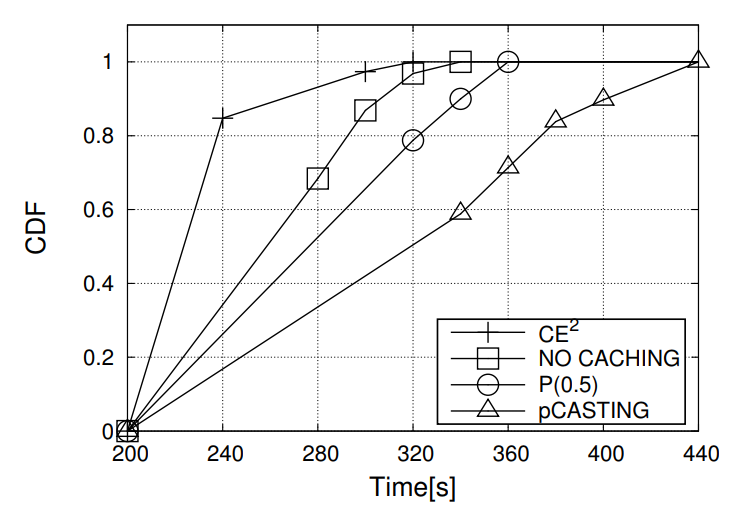
\includegraphics[width=\textwidth]{pix/fig1.PNG}

Cumulative Distribution Function of the discharge time of the nodes in the network.

}



%%% Bild 3 %%%%%%%%%%%%%%%%%%%%%%%%%%%%%%%%%%%%%%%%%%%%%%%%%%%%%%%%%%%%%%%%%%%%%
\headerbox{\textsf{Table 1}}{name=table1, column=3, span=2, below=bild1}{
	
	\centering
	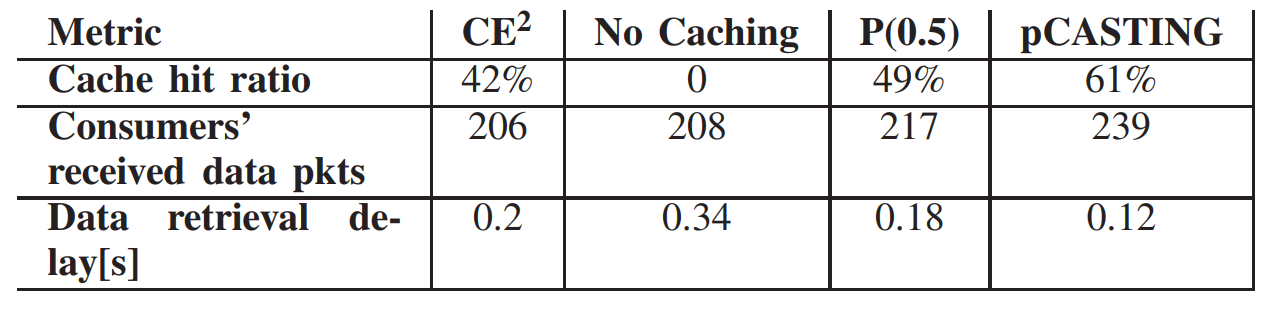
\includegraphics[width=\textwidth]{pix/tab1.PNG}
	
	Data dissemination performance metrics for the different caching strategies.
	
}


%%% Bild 2 %%%%%%%%%%%%%%%%%%%%%%%%%%%%%%%%%%%%%%%%%%%%%%%%%%%%%%%%%%%%%%%%%%%%%
\headerbox{\textsf{Evaluation}}{name=evaluation,column=3, span=2, below=table1}{
\vspace{0.5cm}
\begin{itemize}
	\item Performance of pCASTING was evaluated by simulating 70 mobile nodes as well as fixed Access Point and sensor nodes
	\item Simulations were compared with \textit{Cache Everything Everywhere}, \textit{No Caching}, and \textit{$P(0.5)$} caching strategies
\end{itemize}	

\subsection*{Network Lifetime Analysis}
\begin{itemize}
	\item pCASTING has a beneficial effect on the energy consumption of nodes, i.e. they were operational for longer
	\item Using pCASTING, less radio transmissions in the overall network are needed
\end{itemize}

\subsection*{Retrieval Performance Analysis}
pCASTING performs better in terms of cache hit ratio and data retrieval delays compared to the other evaluated caching strategies.

\begin{itemize}
	\item Data is delivered faster to consumers
	\item Less radio transmissions are neede for data retrieval
\end{itemize}

\vspace{1cm}
}

\headerbox{\textsf{Conclusion}}{name=concl,column=3, span=2, below=evaluation,above=bottom}{
\vspace{0.5cm}

\begin{itemize}
	\item pCASTING proves to be useful in mobile applications of Named Data Networking.
	\item It can be extended to take more parameters and attributes into account and may thus be subject to further research on the topic of caching in Named Data Networks.
\end{itemize}

\vspace{0.5cm}
}




%%% References %%%%%%%%%%%%%%%%%%%%%%%%%%%%%%%%%%%%%%%%%%%%%%%%%%%%%%%%%%%%%%%%%%%%%
\headerbox{\textsf{Quellen}}{name=references, column=0, span=3, above=bottom, below=pcasting}{
  \begin{small}
  \renewcommand{\refname}{\vspace{-0.8em}}
  \setlength{\parskip}{0cm}
  \setlength{\bibsep}{0cm}
  \printbibliography
  \end{small}
}

\end{poster}

\end{document}
